%% START EACH QUESTION WITH A 'section' AND GIVE APPROPRIATE TITLE
\section{ALICE IN WONDERLAND}
	%% FILL IN THE EXPERIMENT NUMBER AND DATE OF COMPLETION
    Experiment Number : 2 \hfill Date : 06-11-2014
	
	%% EACH OF YOUR ROUGH RECORD SECTIONS GO IN HERE AS 'subsection'
	%% AIM IS THE PROBLEM STATEMENT GIVEN TO YOU IN LABS
    \subsection{AIM}
		%% USE 'par' TO DEFINE PARAGRAPHS
		\par Alice and her family are residents of \emph{Wonderland}. One day Alice decided to pay a visit to her uncle who is living in a far away place. She looked up the possible routes using \emph{Google Maps}. She was astounded by the number of paths returned by \emph{Google Maps}. Your task is to help Alice find the least possible amount of money with which she can make the travel to her uncle's home.
		\par The transportation system of \emph{Wonderland} was created in a special way to avoid accidents. All the roads in \emph{Wonderland} are one-way roads. But the roads are designed in such a way that one can reach from a place to any other place.
		
	%% OBJECTIVE WILL GIVE THE UNDERLYING CONCEPT WHICH IS REQUIRED TO IMPLEMENT THE SOLUTION
	\subsection{OBJECTIVE}
		\par The problem at hand can be solved using the Dijkstra's Algorithm for finding the shortest path between two nodes in a graph. The cities in Wonderland can be seen as the nodes and the roads can be seen as the edges.
		\par From the description of the transportation system, it is evident that the edges are directional. Thus, we can use the matrix representation of graph for solving the problem.
		
	%% THEORETICAL BACKGROUND WILL GIVE A BRIEF DESCRIPTION ABOUT THE UNDERLYING CONCEPT AND ITS WORKING
    \subsection{THEORETICAL BACKGROUND}
		\par Dijkstra's algorithm, conceived by computer scientist Edsger Dijkstra in 1956 and published in 1959, is a graph search algorithm that solves the single-source shortest path problem for a graph with non-negative edge path costs, producing a shortest path tree. This algorithm is often used in routing and as a subroutine in other graph algorithms.
		\par For a given source vertex (node) in the graph, the algorithm finds the path with lowest cost (i.e. the shortest path) between that vertex and every other vertex. It can also be used for finding costs of shortest paths from a single vertex to a single destination vertex by stopping the algorithm once the shortest path to the destination vertex has been determined. For example, if the vertices of the graph represent cities and edge path costs represent driving distances between pairs of cities connected by a direct road, Dijkstra's algorithm can be used to find the shortest route between one city and all other cities. As a result, the shortest path algorithm is widely used in network routing protocols, most notably IS-IS and OSPF (Open Shortest Path First).
	
\newpage
	%% PROCEDURE DESCRIBES HOW YOU WILL SOLVE THE GIVEN PROBLEM STATEMENT
	%% USING THE UNDERLYING CONCEPTS
	\subsection{PROCEDURE}
		\par The procedure adopted for implementing the aim is as follows.
		\begin{enumerate}
			\item Read the number of cities, the details of the roads in between them
			\item Read the source and destination cities
			\item Run the Dijkstra's algorithm for these two cities
			\item Return the cost
		\end{enumerate}
	%\newpage %% << USE 'newpage' AT APPROPRIATE PLACES SO THAT ALGORITHMS DO NOT BREAK BETWEEN PAGES
	
	%% GIVE THE ALGORITHMS FOR THE MAJOR OPERATIONS HERE
	\subsection{ALGORITHMS}
	
		%% USE SEPARATE 'subsubsection' FOR EACH ALGORITHM
		\subsubsection{Dijkstra's Algorithm}

%% BEGINNING OF ALGORITHM
\begin{algorithm}
\caption{ : modified\_Dijkstras( $Graph$, $source$, $destination$)} %% << NAME OF THE ALGORITHM WITH PARAMETERS
\begin{algorithmic}[1]  %% << BODY OF ALGORITHM BEGINS
\STATE dist[$source$] := 0
\FORALL{$vertex\ v \in Graph$}
	\IF{$v \neq source$}
		\STATE dist[$v$] := infinity
		\STATE prev[$v$] := undefined
	\ENDIF
	\STATE Q.add\_with\_priority($v$, dist[$v$])
\ENDFOR

\WHILE{Q is not empty}
	\STATE $u$ := Q.extract\_min()
	\STATE mark $u$ as scanned
	\FORALL{neighbor $v$ of $u$}
		\IF{$v$ is not yet scanned}
			\STATE $alt$ = dist[$u$] + length( $u$, $v$ )
			\IF{$alt$ $<$ dist[$v$]}
				\STATE dist[$v$] := $alt$
				\STATE prev[$v$] := $u$
				\STATE Q.decrease\_priority( $v$, $alt$ )
			\ENDIF
		\ENDIF
	\ENDFOR
\ENDWHILE

\RETURN dist[$destination$]
\end{algorithmic}  %% <<BODY OF ALGORITHM ENDS
%% \label{algo:kSelection}
%% << YOU CAN GIVE A LABEL HERE IF YOU WANT TO REFER TO THIS ALGORITHM
%% << LATER IN THE TEXT (USING 'ref')
\end{algorithm}
%% END OF ALGORITHM

%% GIVE A DESCRIPTION ABOUT THE PARAMETERS OF THE ALGORITHM AND THE WORKING
%% IF THE ALGORITHM IS A COMPLEX ONE OR IF THE ALGORITHM IS DEVICED BY YOU
			\par The input parameters to the algorithm are the graph, source and destination. The array $dist[i]$ stores the distance between the source and the corresponding city $i$. The array $prev[i]$ stores the city visited just before the city $i$.
			\par The data structure $Q$ is a priority queue with operations such as $add\_with\_priority$, $decrease\_priority$, etc. The function $length(u,v)$ will give the cost of travelling from city $u$ to $v$.

\newpage
	%% PUT YOUR CODE HERE. IF THE CODE IS TOO LARGE, PASTE ONLY IMPORTANT FUNCTIONS
	%% WHOSE ALGORITHMS YOU HAVE GIVE IN THE ABOVE SECTION
	\subsection{PROGRAM}
	
		%% USE SEPARATE 'subsubsection' FOR EACH FILE
		\subsubsection{Alice.c}
		
			%% SET THE LANGUAGE OF THE CODE USING 'lstset'
			\lstset{language=C}
			
			%% PASTE THE CODE INSIDE THE 'lstlisting' ENVIRONMENT
			%% KEEP THE SOURCE CODE WELL INDENTED AND FORMATTED TO ENSURE READABILITY
			\begin{lstlisting}
#include<stdio.h>
#include<stdlib.h>

#define MAX 1001
#define INF 9999
#define INITIAL 0
#define WAITING 1
#define FINISHED 2

struct node {
	int data;
	int priority;
	struct node *link;
};

int ADJACENT[MAX][MAX];
int DISTANCE[MAX];
int STATUS[MAX];

void init( int );
void dijkstra( int, int, int );
void enqueue( struct node **, struct node **, int , int );
int dequeue( struct node **, struct node ** );
void decrease_priority( struct node **, struct node **, int , int );
int is_empty( struct node * );

int main( int argc, char **argv )
{
	int v1, v2, w, N, s, i, d;
	scanf( "%d", &N );

	init( N );

	while( 1 )
	{
		scanf( "%d %d %d", &v1, &v2, &w );
		if( v1 == -1 && v2 == -1 && w == -1 )
			break;
		if( ADJACENT[v1][v2] > w )
			ADJACENT[v1][v2] = w;
	}

	scanf( "%d %d", &s, &d );

	dijkstra( s, N, d );

	if( DISTANCE[d] < INF )
		printf( "%d\n", DISTANCE[d] );
	else
		printf( "IMPOSSIBLE\n" );

	return 0;
}

void init( int count )
{
	int i, j;
	for( i=1; i<=count; i++ )
	{
		for( j=1; j<=count; j++ )
			if( i != j )
				ADJACENT[i][j] = INF;
		DISTANCE[i] = INF;
		STATUS[i] = INITIAL;
	}
}

void dijkstra( int source, int N, int destination )
{
	struct node *front=NULL, *rear=NULL;
	int i, v, alt;

	DISTANCE[source] = 0;
	for( i=1; i<=N; i++ )
	{
		if( STATUS[i] == INITIAL )
		{
			enqueue( &front, &rear, i, DISTANCE[i] );
			STATUS[i] = WAITING;
		}
	}

	while( !is_empty( front ) )
	{
		v = dequeue( &front, &rear );
		STATUS[v] = FINISHED;

		if( v == destination )
			return;

		for( i=1; i<=N; i++ )
		{
			if( ADJACENT[v][i] != INF && STATUS[i] == WAITING )
			{
				alt = DISTANCE[v] + ADJACENT[v][i];
				if( alt < DISTANCE[i] )
				{
					DISTANCE[i] = alt;
					decrease_priority( &front, &rear, i, alt );
				}
			}
		}
	}
}

void enqueue( struct node **frontp, struct node **rearp, int data, int priority )
{
	struct node *new_node = (struct node *)malloc(sizeof(struct node));
	new_node->data = data;
	new_node->priority = priority;
	new_node->link = NULL;

	if( *rearp == NULL )
		*frontp = *rearp = new_node;
	else if( priority <= (*frontp)->priority )
	{
		new_node->link = *frontp;
		*frontp = new_node;
	}
	else if( priority >= (*rearp)->priority )
	{
		(*rearp)->link = new_node;
		*rearp = new_node;
	}
	else
	{
		struct node *parent = *frontp, *temp = (*frontp)->link;

		while( temp != NULL && temp->link != NULL && temp->priority < priority )
		{
			parent = temp;
			temp = temp->link;
		}
		parent->link = new_node;
		new_node->link = temp;
	}
}

int dequeue( struct node **frontp, struct node **rearp )
{
	int data = (*frontp)->data;
	*frontp = (*frontp)->link;
	if( *frontp == NULL )
		*rearp = NULL;
	return data;
}

void decrease_priority( struct node **frontp, struct node **rearp, int data, int priority )
{
	struct node *p = *frontp, *t=(*frontp)->link;
	if( t == NULL || p->data == data )
		p->priority = priority;
	else
	{
		while( t->data != data )
		{
			p = t;
			t = t->link;
		}
		p->link = t->link;
		enqueue( frontp, rearp, data, priority );
	}
}

int is_empty( struct node *front )
{
	if( front == NULL )
		return 1;
	return 0;
}
\end{lstlisting}
\newpage

	%% TAKE SCREENSHOT OF THE OUTPUT AND PUT IT HERE
	\subsection{SAMPLE OUTPUT}
		\begin{figure}[ht] 
			\centering
			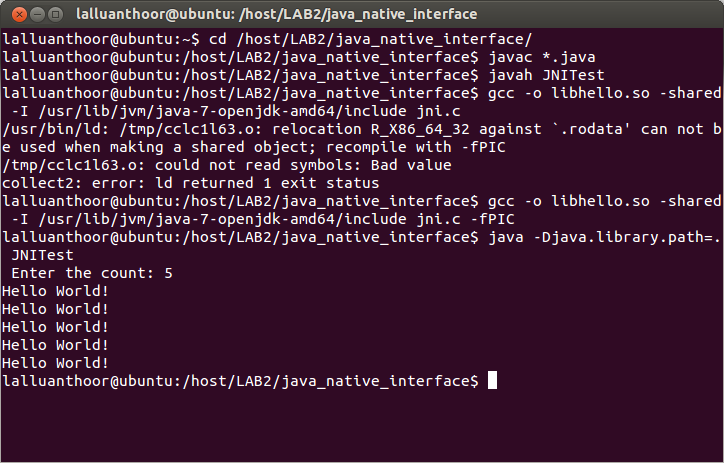
\includegraphics[width=\textwidth]{jni_op.png}
			\caption{Screen-shot of Output}
		\end{figure} 

	%% RESULT IS OBTAINED/SPECIFIED REGARDING THE PROBLEM DEFINITION OR AIM
	\subsection{RESULT}
		\par The least possible ticket cost for Alice to reach her uncle's home is found out and displayed.
	
	%% INFERENCE IS OBTAINED/SPECIFIED REGARDING THE OBJECTIVE AND PROCEDURE
	\subsection{INFERENCES}
		\par The Single Source Shortest Path algorithm deviced by Dijkstra was implemented using C. The graph was represented using adjacency matrix and the Dijkstra's algorithm was implemented using a \emph{Priority Queue}.

\newpage  %% << END YOUR PROGRAM WITH A 'newpage' COMMAND